
\newpage
\section{Задание 6}
{\bf\large Условие}\\
Из полосы жести шириной $a$ требуется сделать открытый сверху
желоб, поперечное сечение которого должно иметь форму равнобочной
трапеции. Дно желоба имеет ширину $b$. Какова должна быть ширина
желоба наверху, чтобы он вмещал наибольшее количество воды? \\
\\
{\bf\large Ход решения}
\begin{center}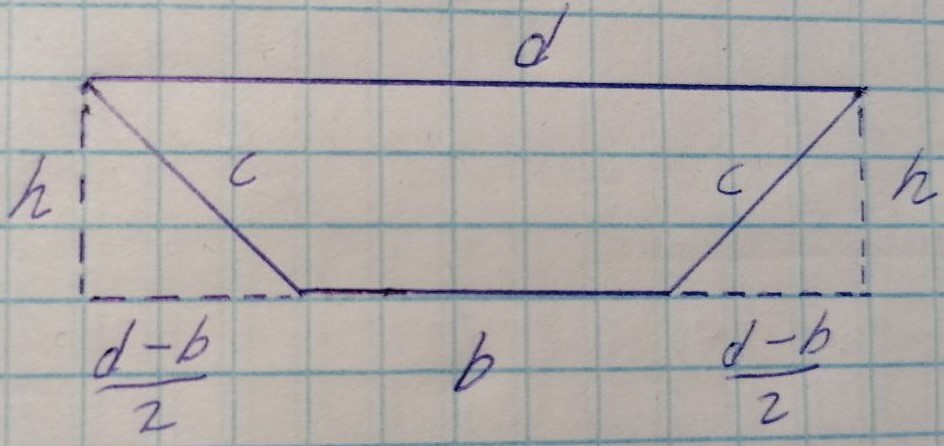
\includegraphics[width=0.7\linewidth]{6.jpg}\end{center}
Где $c = \frac{a-b}{2}$. \\
По теореме Пифагора: $c^2 = h^2 + \left(\frac{d-b}{2}\right)^2 \Rightarrow \left(\frac{a-b}{2}\right)^2 = h^2 + \left(\frac{d-b}{2}\right)^2
\Rightarrow h = \sqrt{\frac{(a-b)^2-(d-b)^2}{4}} = \sqrt{\frac{a^2-2ab-d^2+2db}{4}}$ \\
Площадь трапеции: $S = \frac{b+d}{2}\cdot h = \frac{b+d}{2} \cdot \sqrt{\frac{a^2-2ab-d^2+2db}{4}}$ \\
Желоб будет вмещать наибольший объем воды при фиксированной длине, если площадь сечения (трапеции) будет максимальной, найдем это максимальное значение с помощью производной: \\
$S' = \frac{1}{2} \sqrt{\frac{a^2-2ab-d^2+2db}{4}} + \frac{b+d}{2} \cdot \frac{-2d+2b}{4} \cdot \frac{1}{2} \cdot \frac{1}{\sqrt{\frac{a^2-2ab-d^2+2db}{4}}}$ \\
Из построения видно, что если $d \rightarrow a-$ то объем воды $=0$. 
К тому же, если $d\rightarrow0+$ то трапеция будет стремится к треугольнику, у которого площадь явно меньше. 
Значит, максимальное значение $S(d)$ будет в какой-нибудь точке локального максимума, найдем их: \\
\linebreak
\noindent Случай 1 ($S'(d)$ - не существует): \\
То есть $\frac{a^2-2ab-d^2+2db}{4}\leq0 \Rightarrow -d^2 + 2db +a^2-2ab\leq 0 \Rightarrow -(d-a)(d+a-2b)\leq 0 \Rightarrow (d-a)(d+a-2b)\geq 0$ \\
Откуда, по методу интерваллов получим, что либо $d\geq a$, либо $d\leq 2b-a$. \\
Первое невозможно так как если $d\geq a$, то трапецию не построишь (даже если боковые стороны "выпрямим" \space к основанию, то их все равно не хватит, чтобы достать до концов отрезка длиной d). \\
А $d\leq 2b-a\Leftrightarrow b+2c \leq 2b -d \Leftrightarrow c \leq \frac{b -d}{2} \Rightarrow c^2 \leq \left(\frac{b -d}{2}\right)^2 \Leftrightarrow \left(\frac{d-b}{2}\right)^2+h^2 \leq \left(\frac{b -d}{2}\right)^2 \Leftrightarrow h^2 \leq 0$ - чего не может быть. 
\newpage
\noindent Случай 2 ($S'(d) = 0$ ): \\
\begin{gather*}
    \frac{1}{2} \sqrt{\frac{a^2-2ab-d^2+2db}{4}} + \frac{b+d}{2} \cdot \frac{-2d+2b}{4} \cdot \frac{1}{2} \cdot \frac{1}{\sqrt{\frac{a^2-2ab-d^2+2db}{4}}} = 0 \\
    \sqrt{\frac{a^2-2ab-d^2+2db}{4}} = \frac{b+d}{2} \cdot \frac{d-b}{2} \cdot \frac{1}{\sqrt{\frac{a^2-2ab-d^2+2db}{4}}} \\
    \left(\sqrt{\frac{a^2-2ab-d^2+2db}{4}}\right)^2 = \frac{(d^2-b^2)}{4}\\
    a^2-2ab-d^2+2db= (d^2-b^2)\\
    2d^2-2bd-(a-b)^2=0
\end{gather*}
Решим квадратное уравнение относительно $d$:
\begin{gather*}
    D = 4b^2+8(a-b)^2 \text{ - сумма квадратов всегда неотрицательна}\\
    d_1 = \frac{2b+\sqrt{4b^2+8(a-b)^2}}{4}\\
    d_2 = \frac{2b-\sqrt{4b^2+8(a-b)^2}}{4} \text{ - явно меньше нуля, чего не может быть}
\end{gather*}
Итого $d = \frac{2b+\sqrt{4b^2+8(a-b)^2}}{4}$, докажем, что это максимум взяв, например $S'\left(\frac{b}{2}\right)$ и $S'\left(\frac{a-b}{\sqrt{2}}+b\right)$ \\
Расчеты, пожалуй опустим ;)\\
{\bf Ответ:} $d = \frac{2b+\sqrt{4b^2+8(a-b)^2}}{4}$
